\documentclass[twoside]{article}


\usepackage[sc]{mathpazo} % Use the Palatino font
\usepackage[T1]{fontenc} % Use 8-bit encoding that has 256 glyphs
\linespread{1.05} % Line spacing - Palatino needs more space between lines
\usepackage{microtype} % Slightly tweak font spacing for aesthetics

\usepackage[hmarginratio=1:1,top=32mm,columnsep=20pt]{geometry} % Document margins
\usepackage{multicol} % Used for the two-column layout of the document
\usepackage[hang, small,labelfont=bf,up,textfont=it,up]{caption} % Custom captions under/above floats in tables or figures
\usepackage{booktabs} % Horizontal rules in tables
\usepackage{float} % Required for tables and figures in the multi-column environment - they need to be placed in specific locations with the [H] (e.g. \begin{table}[H])
\usepackage{hyperref} % For hyperlinks in the PDF

\usepackage{lettrine} % The lettrine is the first enlarged letter at the beginning of the text
\usepackage{paralist} % Used for the compactitem environment which makes bullet points with less space between them

\usepackage{titlesec} % Allows customization of titles
\renewcommand\thesection{\Roman{section}} % Roman numerals for the sections
\renewcommand\thesubsection{\Roman{subsection}} % Roman numerals for subsections
\titleformat{\section}[block]{\large\scshape\centering}{\thesection.}{1em}{} % Change the look of the section titles
\titleformat{\subsection}[block]{\large}{\thesubsection.}{1em}{} % Change the look of the section titles

\usepackage{fancyhdr} % Headers and footers
\pagestyle{fancy} % All pages have headers and footers
\fancyhead{} % Blank out the default header
\fancyfoot{} % Blank out the default footer
\fancyhead[C]{USC EE511-PROJECT1} % Custom header text
\fancyfoot[RO,LE]{\thepage} % Custom footer text



\usepackage{multicol}
\usepackage{listings}
\usepackage{graphicx}
\usepackage{caption}
\usepackage{subcaption}
\usepackage{hyperref}
\usepackage{color}
\usepackage{float}
\usepackage{mathtools}
\usepackage{amssymb}
\usepackage{wrapfig}

%----------------------------------------------------------------------------------------
%	TITLE SECTION
%----------------------------------------------------------------------------------------

\title{\vspace{-15mm}\fontsize{24pt}{10pt}\selectfont\textbf{Project \#1 - Coin flip }} % Article title

\author{
\large
\textsc{Li Yicheng}\thanks{\href{https://github.com/IAMLYCHEE/EE511-PROJECT1}{github link: https://github.com/IAMLYCHEE/EE511-PROJECT1} }\\[2mm] % Your name
\normalsize USCID:7827077047\\
\normalsize email: l.y.c.liyicheng@gmail.com \\ % Your institution
\normalsize USC Viterbi of Engineering
\vspace{-5mm}
}

\date{}

%----------------------------------------------------------------------------------------

\begin{document}

\maketitle % Insert title

\thispagestyle{fancy} % All pages have headers and footers

\section{Simulation of the Bernoulli Outcomes ---- Q1}
\textbf{1.Requirement}: tossing a fair coin 50 times. Count the number of heads. Record the longest run of heads. Generate a histogram for the Bernoulli outcomes.\\ \\
\textbf{2.Tool}: Matlab (Version: R2014b Platform: Ubuntu 16.04 LTS)\\ \\
\textbf{3.Experiment}: For further experiment convenience, I generated a function for the experiment trial. In the function, a coin (can be either fair or biased ) is tossed several times. The amount of trial is determined by the input parameter eval\_budget and the coin property(fair or not) is determined by the parameter p\_thre. The output is the head number and the longest run of the head. This function also plot the histogram showing the number of heads and tails plus a figure showing the relative frequency througout the experiment. \\ \\
\textbf{4.core code:}
% \begin{multicols}{2}
\lstset{ %
language=Matlab,                % choose the language of the code
basicstyle=\footnotesize,       % the size of the fonts that are used for the code
numbers=left,                   % where to put the line-numbers
numberstyle=\footnotesize,      % the size of the fonts that are used for the line-numbers
stepnumber=1,                   % the step between two line-numbers. If it is 1 each line will be numbered
numbersep=5pt,                  % how far the line-numbers are from the code
backgroundcolor=\color{white},  % choose the background color. You must add \usepackage{color}
showspaces=false,               % show spaces adding particular underscores
showstringspaces=false,         % underline spaces within strings
showtabs=false,                 % show tabs within strings adding particular underscores
frame=single,           % adds a frame around the code
tabsize=2,          % sets default tabsize to 2 spaces
captionpos=b,           % sets the caption-position to bottom
breaklines=true,        % sets automatic line breaking
breakatwhitespace=false,    % sets if automatic breaks should only happen at whitespace
escapeinside={\%*}{*)}          % if you want to add a comment within your code
}
\begin{lstlisting}
function [head_number,longest_run] = tossing_coin(eval_budget,p_thre)
% usage: function [head_number,longest_run] = tossing_coin(eval_budget,p_thre)
%tossing eval_budget times
%Author : Li Yicheng 

%define variables
result = zeros(eval_budget,1);
length = 0;
longest_run = 0;
head_number = 0;
tail_number = 0;
head_rela_fre = zeros(1,eval_budget);
tail_rela_fre = zeros(1,eval_budget);
for i = 1 : eval_budget
    coin = rand(1) < p_thre;
    if coin > 0 % a head
        head_number = head_number + 1;
        length = length + 1; %add length
        result(i) = 1;
        %the state now is a head
    else % a tail
        tail_number= tail_number + 1;
        result(i) = 0;
        if length > longest_run
            longest_run = length; %refresh the new longest run
        end
        length = 0; %reset the length
        %the state now is a tail
    end
        head_rela_fre(i) = head_number / i;
        tail_rela_fre(i) = tail_number / i;
end
\end{lstlisting}
% \end{multicols}
\textbf{5.result}: Executing query: tossing\_coin(50,0.5)

\begin{figure}[H]%  figure placement: here, top, bottom, or page
   \centering
   \begin{subfigure}[b]{0.47\textwidth}
   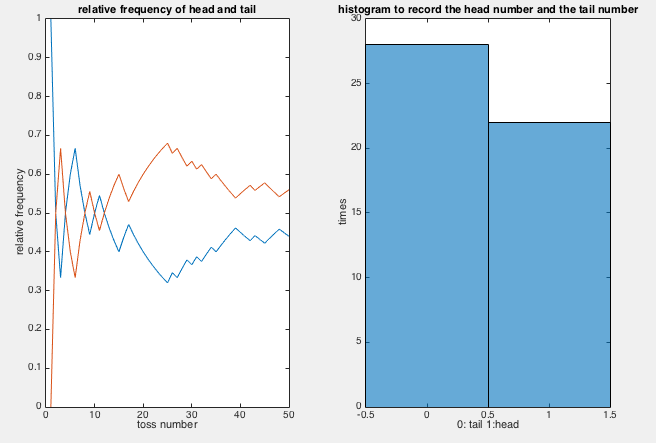
\includegraphics[width=\textwidth]{../data/exp1.png} 
   \caption{toss 50 times}
   % \label{fig:example3}
   \end{subfigure}
   ~
   \begin{subfigure}[b]{0.47\textwidth}
   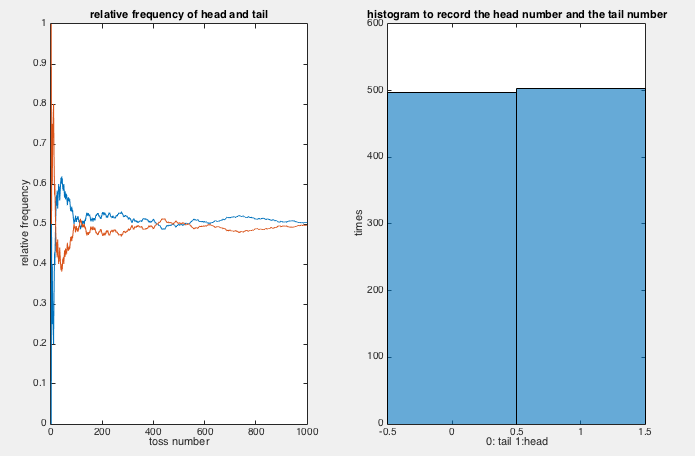
\includegraphics[width=\textwidth ]{../data/exp1_e.png} 
   \caption{toss 1000 times}
   % \label{fig:example3}
   \end{subfigure}


   \caption{left: change of relative frequency , \t right: histogram of the Bernoulli Outcome}
\end{figure}
from the figure1(a), the experiment ends with 28 heads and 22 tails and let's toss the coin 1000 times by calling tossing\_coin(1000,0.5), and we got the figure1(b). And from the result we can say with a far more larger amount of trials given, the relative frequency of heads and tail both have a convergency to 0.5. In this experiment, the longest run of heads is 6.\\ \\

\section{Number of Heads Experiment ---- Q1.a}
\textbf{1.Requirement}: Repeat the first experiment 20,100,200, and 1000 times. Count the number of heads in 50 flips. Generate a histogram showing the phenomenon.\\ \\
\textbf{2.Tool}: Matlab (Version: R2014b Platform: Ubuntu 16.04 LTS)\\ \\
\textbf{3.Experiment}: Since this time we only care about the result of the amount of heads, we only need the sum of the result vector (0 is tail and 1 is head, therefore the sum of the vector is the number of the heads in 50 flips). Then we generate a histogram showing what is the most frequent number of head we would get.\\ \\
\textbf{4.core code}:
% \begin{multicols}{2}
\lstset{ %
language=Matlab,                % choose the language of the code
basicstyle=\footnotesize,       % the size of the fonts that are used for the code
numbers=left,                   % where to put the line-numbers
numberstyle=\footnotesize,      % the size of the fonts that are used for the line-numbers
stepnumber=1,                   % the step between two line-numbers. If it is 1 each line will be numbered
numbersep=5pt,                  % how far the line-numbers are from the code
backgroundcolor=\color{white},  % choose the background color. You must add \usepackage{color}
showspaces=false,               % show spaces adding particular underscores
showstringspaces=false,         % underline spaces within strings
showtabs=false,                 % show tabs within strings adding particular underscores
frame=single,           % adds a frame around the code
tabsize=2,          % sets default tabsize to 2 spaces
captionpos=b,           % sets the caption-position to bottom
breaklines=true,        % sets automatic line breaking
breakatwhitespace=false,    % sets if automatic breaks should only happen at whitespace
escapeinside={\%*}{*)}          % if you want to add a comment within your code
}
\begin{lstlisting}
function repeat_trial(trial_time)
%usage: repeat_trial(trail_time)
%Li Yicheng
%repeat the 50 tossing coin trial several times
for i = 1 : trial_time % repeat trial_time 
    result  = rand(1,50); %generate the result
    exp_trial(i) = sum(result);%count the number of heads and store the amount
end
histogram(exp_trial,50,'BinLimits',[0,50]) %plot the result of the experiment
title('exp_trial times')
xlabel('number of heads')
ylabel('times')
\end{lstlisting}
% \end{multicols}
\textbf{5.result}: 

\begin{figure}[H]%  figure placement: here, top, bottom, or page
   \centering
   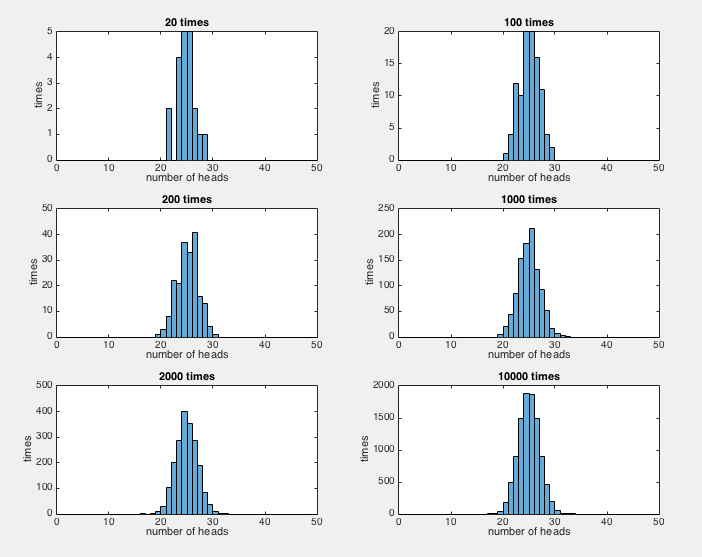
\includegraphics[scale = 0.6]{../data/exp1_a.png} 
   \caption{number of heads histogram}  
\end{figure}
Observation: we can see that we got four `mountains' in figure2. when the trial time increase to 1000, the peak of the mountain is somewhere near 25 and the number of heads has the highest probability to vary between 23 to 27. This is quite easy to get for a fair coin, because there is no biase on head over tail. When we assigned a large number 10000 to this experiment we saw a fairly symmetric mountain. Both side decline in a regular way. Mathematically, this situation can be computed. The probability to get 25 heads is $\binom {50}{25} (0.5)^{25}\cdot 0.5^{25}$, the 26 heads probability is $\binom {50}{26} (0.5)^{26}\cdot (0.5)^{24} $ and $P(25heads) / P(26heads) = 26 / 25$ generally $\binom nk / \binom{n}{k+1} = (k+1)/(n-k)$ so it will decrease faster and faster. 

\section{Biased Coin Experiment ---- Q2}
\textbf{1.Requirement}: Simulate tossing a biased coin 200 times where P(HEAD) = 0.8. Count the number of heads. Record the longest run of heads. Generate a histogram for the outcomes.\\ \\
\textbf{2.Tool}: Matlab (Version: R2014b Platform: Ubuntu 16.04 LTS)\\ \\
\textbf{3.Experiment}: Using the tossing\_coin function again in Q1, query tossing\_coin(200,0.8). Two figures are derived one is the tendency of the relative frequency and the other is the histogram showing the number of heads and tails, the same as the first experiment.\\ \\
\textbf{4.result}:\\
\begin{wrapfigure}{l}{0.6\textwidth}%  figure placement: here, top, bottom, or page
   \begin{center}
   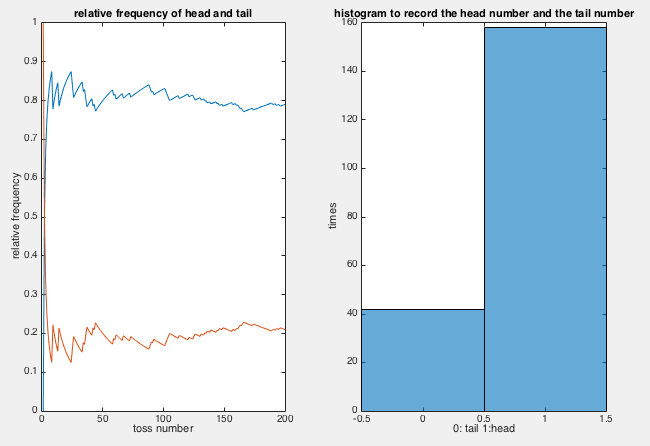
\includegraphics[scale = 0.35]{../data/exp2.png}
   \end{center} 
   \caption{number of heads histogram} 
   \vspace{20pt} 
\end{wrapfigure}
\\
Figure3 shows the result of tossing a biased coin, the relative frequency of heads has a convergency to 0.8, the number of heads is nearly 160 which is the 80\% of 200.\\ \\ \\ \\

\section{Head Run Length Experiment ---- Q3}
\textbf{1.Requirement}: Simulating tossing a fair coin 100 times. Generate a histogram showing the heads run length.\\ \\
\textbf{2.Tool}: Matlab (Version: R2014b Platform: Ubuntu 16.04 LTS)\\ \\
\textbf{3.Experiment}: Construct a function called head\_run with the input parameter tossing times named eval\_budget. To do this experiment by calling head\_run(100).\\ \\
\textbf{4.Core Code}:\\
 \lstset{ %
language=Matlab,                % choose the language of the code
basicstyle=\footnotesize,       % the size of the fonts that are used for the code
numbers=left,                   % where to put the line-numbers
numberstyle=\footnotesize,      % the size of the fonts that are used for the line-numbers
stepnumber=1,                   % the step between two line-numbers. If it is 1 each line will be numbered
numbersep=5pt,                  % how far the line-numbers are from the code
backgroundcolor=\color{white},  % choose the background color. You must add \usepackage{color}
showspaces=false,               % show spaces adding particular underscores
showstringspaces=false,         % underline spaces within strings
showtabs=false,                 % show tabs within strings adding particular underscores
frame=single,           % adds a frame around the code
tabsize=2,          % sets default tabsize to 2 spaces
captionpos=b,           % sets the caption-position to bottom
breaklines=true,        % sets automatic line breaking
breakatwhitespace=false,    % sets if automatic breaks should only happen at whitespace
escapeinside={\%*}{*)}          % if you want to add a comment within your code
}
\begin{lstlisting}
function head_run(eval_budget)
% usage: function head_run(eval_budget)
% Li Yicheng
% record the heads run 
head_number = 0;
length = 0; %to store the number of heads run length
j = 1; %store the index of the record, every time a continous series of heads end, j plus one to its self for another record.
for i = 1 : eval_budget %toss eval_budget times
    coin = rand(1) > 0.5; % a fair coin
    if coin > 0 %a head
        head_number = head_number + 1;
        length = length + 1; %add length
    else % a tail
        if length > 0
            record(j) = length;  %record the head run
            j = j + 1;
        end
        length = 0; %reset the length
    end
end
histogram(record')
title('histogram for the outcome')
title('the histogram of the run length of head')
xlabel('run length')
ylabel('times')
\end{lstlisting}
\textbf{5.result}: \\

\begin{wrapfigure}{l}{0.55\textwidth}%  figure placement: here, top, bottom, or page
   \begin{center}
   \begin{subfigure}{0.55\textwidth}
   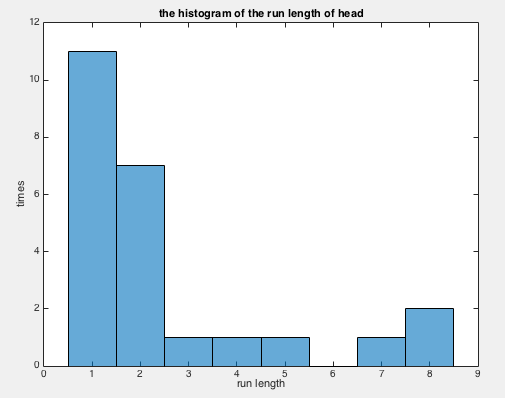
\includegraphics[scale = 0.45]{../data/exp3.png}
   \caption{tossing 100 times}
   \end{subfigure}
   ~
   \begin{subfigure}{0.55\textwidth}
   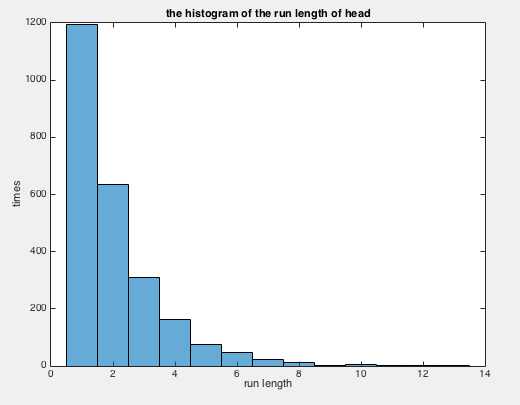
\includegraphics[scale = 0.45]{../data/exp3_e.png}
   \caption{tossing 10000 times}
   \end{subfigure}
   \end{center} 
   \caption{number of heads histogram}  
   \vspace{-20pt}
\end{wrapfigure} 
From the figure4(a) we can see that the run length has the largest posiibility to be one or two and the longest run length is 8. Let's make an assumption that this is also true when we tossing a coin 10000 times. let's excuting a query of head\_run(10000).
Not surprisingly, we have the longest run length of only 13 and we have the most frequent length of 1, 2 and 3. Therefore, the conclusion is that it is hard for the head condition can not maintain for a long time. Moreover, if we take a look at the figure 5, we saw a `regular' downstair. If we use the knowledge of probability to describe what we saw in figure 4(b), every toss is a i.i.d.(independent and identically distributed) experiment. So we get the run length of 1 with the probabilty 0.5, and 2 with 0.25, 3 with $1/2 \cdot 1/2 \cdot 1/2 = 1/8$ . The figure 4(b) seems to arrive at the similar result. 
\clearpage
\newpage
\section{Reach Specified amount of Heads ---- Q4}
\textbf{1.Requirement}: Simulate tossing a fair coin and count the number of tosses until reaching a user-specified possitive number of heads.\\ \\
\textbf{2.Tool}: Matlab (Version: R2014b Platform: Ubuntu 16.04 LTS)\\ \\
\textbf{3.Experiment}: Just use the while loop in the code design and the loop break until the requirement is met. Use a table to record the data. Query the function toss\_until(p\_thre)\\ \\
\textbf{4.Core Code}: \\
 \lstset{ %
language=Matlab,                % choose the language of the code
basicstyle=\footnotesize,       % the size of the fonts that are used for the code
numbers=left,                   % where to put the line-numbers
numberstyle=\footnotesize,      % the size of the fonts that are used for the line-numbers
stepnumber=1,                   % the step between two line-numbers. If it is 1 each line will be numbered
numbersep=5pt,                  % how far the line-numbers are from the code
backgroundcolor=\color{white},  % choose the background color. You must add \usepackage{color}
showspaces=false,               % show spaces adding particular underscores
showstringspaces=false,         % underline spaces within strings
showtabs=false,                 % show tabs within strings adding particular underscores
frame=single,           % adds a frame around the code
tabsize=2,          % sets default tabsize to 2 spaces
captionpos=b,           % sets the caption-position to bottom
breaklines=true,        % sets automatic line breaking
breakatwhitespace=false,    % sets if automatic breaks should only happen at whitespace
escapeinside={\%*}{*)}          % if you want to add a comment within your code
}
\begin{lstlisting}
function num_tosses = toss_until(p_thre)
%usage: function num_tosses = toss_until(p_thre)
%Author: Li Yicheng
num_wanted = input('the number of heads you want:');
head_number = 0;
num_tosses = 0;
while (head_number < num_wanted)
    num_tosses = num_tosses + 1;
    if rand(1) > p_thre %a head occurs
        head_number = head_number + 1;
    end
end
\end{lstlisting}
\textbf{5.result}:\\ \\ 
\begin{tabular}{|| c | c ||}
 \hline \hline
 heads query & trial amount \\ \hline \hline
20 & 45 \\ \hline
50 & 110 \\ \hline
100 & 189 \\ \hline
200 & 407 \\ \hline
500 & 1024 \\ \hline
1000 & 1984 \\ \hline
\end{tabular}
\\ \\
The results show that we need nearly twice the number of the expected amount of heads trials. And for a fair coin, this result is rational because the probabilty to get a head is 50\%.

\end{document}